%!TEX TS-program = ./make.zsh

\documentclass[a4paper,12pt]{article}

\title{The Effect of Hole Ice on the Propagation and Detection of Light in IceCube}
\author{Sebastian Fiedlschuster}
\newcommand\shorttitle{Hole Ice}
\newcommand\entwurf{\today}

% TODO: Customze layout here.

\usepackage{microtype}
\usepackage{parskip}

\usepackage[T1]{fontenc}
\usepackage[utf8]{inputenc}
\usepackage{lipsum}
\usepackage{graphicx}
\usepackage[font=footnotesize]{caption}

\newcommand\image[1]{\includegraphics[width=\textwidth]{img/#1}}
\newcommand\smallerimage[1]{\centering\includegraphics[width=0.6\textwidth]{img/#1}}
\newcommand\halfimage[1]{\includegraphics[width=0.48\textwidth]{img/#1}}
\newcommand\halfcropimage[2]{\includegraphics[width=0.48\textwidth, trim={#2}, clip]{img/#1}}
\newcommand\thirdimage[1]{\includegraphics[width=0.32\textwidth]{img/#1}}

\newcommand\fig[2]{
  \begin{figure}[htb]
    \begin{margincap}
      \centering
      \image{#1}
      \caption{#2}
    \end{margincap}
  \end{figure}
}

\usepackage{placeins} % implements \FloatBarrier

\usepackage{fontawesome}

\usepackage[font=scriptsize, position=b]{subcaption}

% http://pgfplots.sourceforge.net/pgfplots.pdf
\usepackage{pgfplots}
% Pandoc (http://pandoc.org) is used in the `Makefile' to pre-process
% `text/*.md.tex` files from markdown to latex. This way, one may use
% lists, section headings etc. in the .md.tex files.

% Pandoc requires a `\tightlist`.
% https://tex.stackexchange.com/a/258486/70789
\providecommand{\tightlist}{%
  \setlength{\itemsep}{0pt}\setlength{\parskip}{0pt}}
% Markierungen mit `\todo{foo}`, `\mref{schiller}`, `\frage{foo}` einfügen.

\usepackage{color}

% Markierung einfügen (Kommentar während der Bearbeitung) % Parameter: Art, Kommentar
\newcommand{\markierung}[2]{
        \textcolor{red}{\textbf{#1:} #2} \\
}

\newcommand{\todo}[1]{\markierung{To do}{#1}} % ToDo-Kommentar einfügen, Parameter: Kommentar
\newcommand{\mref}[1]{\markierung{Verweis einfügen}{#1}} % Fehlenden Verweis markieren, Parameter: Kommentar
\newcommand\frage[1]{\markierung{Frage}{#1}} % Frage

\usepackage[backend=biber]{biblatex}

\usepackage{amsmath}
\usepackage{amssymb}

% Vectors
\renewcommand{\vec}[1]{\overrightarrow{#1}}
\newcommand{\norm}[1]{\left\lVert#1\right\rVert}
\newcommand{\len}[1]{\overline{#1}}

% Comparison operators
\newcommand{\identical}{\equiv}

% Sets
\newcommand{\reals}{\mathbb{R}}
\newcommand{\naturals}{\mathbb{N}}

% Constants
\newcommand{\e}{\mathrm{e}}
% Highlighted code listings, https://ctan.org/pkg/minted
%
% This requires pygments.
%
%     pip install Pygments
%     cd /Library/TeX/texbin
%     sudo ln -s `which pygmentize` pygmentize
%     sudo tlmgr install fvextra
%     sudo tlmgr update minted
%
\usepackage[outputdir=./build]{minted}

\setminted{
  tabsize=2, linenos, breaklines, autogobble, breakautoindent, frame=lines, framesep=2mm
}

\newenvironment{python}{\minted{python}}{\endminted}
\newcommand\pythoninput[1]{\inputminted{python}{#1}}

\newenvironment{ccode}{\minted{c}}{\endminted}
\newcommand\appendixref[1]{appendix \ref{#1}, p.\,\pageref{#1}}
\usepackage[ngerman, english]{babel}

\usepackage{iflang}

\IfLanguageName{ngerman}{
  \newcommand\pageStr{Seite}
}{
  \newcommand\pageStr{Page}
}
\usepackage[explicit]{titlesec}

% The current section, subsection and subsubsection
% are stored in these commands, such that they can
% be included in the page header.
%
\newcommand\currentsection{}
\newcommand\currentsubsection{}
\newcommand\currentsubsubsection{}

% \preparesectionmarks needs to be called after \pagestyle in order to
% copy the current section titles into the header.
% https://de.wikibooks.org/wiki/LaTeX-Wörterbuch:_chaptermark
%
\newcommand\preparesectionmarks{
  \renewcommand\sectionmark[1]{\renewcommand\currentsection{##1}}
  \renewcommand\subsectionmark[1]{\renewcommand\currentsubsection{##1}}
  \renewcommand\subsubsectionmark[1]{\renewcommand\currentsubsubsection{##1}}
}

% http://tug.ctan.org/macros/latex/contrib/titlesec/titlesec.pdf
% https://tex.stackexchange.com/a/59727/70789
%
% \titleformat{⟨command⟩}[⟨shape⟩]{⟨format⟩}{⟨label⟩}{⟨sep⟩}{⟨before-code⟩}[⟨after-code⟩]
%\titleformat{\section}{\Large\bfseries}{\thesection\quad}{0cm}{\renewcommand{\currentsection}{#1} #1}
%\titleformat{\subsection}{\large\bfseries}{\thesubsection\quad}{0cm}{\renewcommand{\currentsubsection}{#1}#1}
%\titleformat{\subsubsection}{\normalsize\bfseries}{\thesubsubsection\quad}{0cm}{\renewcommand{\currentsubsubsection}{#1}#1\emph{}}

% Start sections on odd pages:
% https://tex.stackexchange.com/a/51926/70789
%
\let\oldsection\section
\def\section{\cleardoublepage\oldsection}
% This file is responsible for the page header.

\usepackage{fancyhdr}

\pagestyle{fancy}
\fancyhf{}

% This provides \currentsection, \currentsubsection and \currentsubsubsection.
% See: lib/section.tex
%
\preparesectionmarks

\fancyhead[L,EL]{%
  \footnotesize
  \minipage{10cm}%
    \textsf{%
      \textbf{{\dokumententitel}},
			\dokumentid,
			\ifthenelse{\equal{\entwurf}{}}{
				\datum
			}{
				\textcolor{red}\entwurf\normalcolor
			} \\
			\ifthenelse{\equal{\currentsubsection}{}}{}{\thesubsection \ \ }\currentsection\ifthenelse{\equal{\currentsubsection}{}}{}{: \currentsubsection}
		}
  \endminipage
}

\fancyhead[C]{}

\fancyhead[OR]{\logo}

\renewcommand{\headrulewidth}{0.0pt} %obere Trennlinie
\addtolength{\headheight}{2\baselineskip} % noch etwas Platz

\fancyfoot[OL]{}
\fancyfoot[C]{}
\fancyfoot[OR,EL]{\vspace{2cm}\fancyfootfont{ Seite \thepage}}

\renewcommand{\footrulewidth}{0.0pt} %untere Trennlinie
\usepackage{xspace}

\newcommand\unit[1]{\text{\,#1}\xspace}
\newcommand\m{\unit{m}}
\newcommand\cm{\unit{cm}}
\newcommand\mm{\unit{mm}}

\newcommand\ns{\unit{ns}}

\usepackage{siunitx}
\usepackage{physics}
\usepackage{hepnames}


% Differentials
\renewcommand\d{\text{d}}
\newcommand\dx{\d x}
\newcommand\dn{\d n}

% Quantities
\newcommand\abs{_\text{abs}}
\newcommand\sca{_\text{sca}}
\newcommand\esca{_\text{e}}
\newcommand\hi{^\text{H}}
\newcommand\lambdaabs{\lambda\abs}
\newcommand\dom{_\text{DOM}}
\newcommand\domhi{_\text{DOM,HI}}
\newcommand\domdima{_\text{DOM,HI}^\text{Dima}}

% Reference to issues on the cd rom and on the web
\newcommand\issue[1]{\texttt{issues/#1} on the cdrom as well as online at \url{https://github.com/fiedl/hole-ice-study/issues/#1}}
\newcommand\script[1]{\texttt{hole-ice-study/scripts/#1} on the cdrom as well as online at \url{https://github.com/fiedl/hole-ice-study/tree/master/scripts/#1}}

% Follow-up marker, not sure how to use this, yet.
\newcommand\followup{}

% Special names
\newcommand\authorname[1]{\noun{#1}\xspace}
\newcommand\softwarename[1]{\noun{#1}\xspace}
\newcommand\clsim{\softwarename{clsim}}
\newcommand\ppc{\softwarename{ppc}}
\newcommand\photonics{\softwarename{Photonics}}
\newcommand\steamshovel{\softwarename{Steamshovel}}
\newcommand\rongen{\authorname{Rongen}}
\newcommand\chirkin{\authorname{Chirkin}}

% Hole-ice parameters
\newcommand\HH{\mathcal{H}}

\includeonly{text/propagation_through_different_media}

\bibliography{diplomarbeit}
\begin{document}
  \maketitle

  \newpage
  \setcounter{tocdepth}{2}
  \tableofcontents

  \section{Introduction}
\label{sec:intro}

\icecube is a neutrino observatory located at Earth's South Pole. It
uses a cubic-kilometer of glacial ice as detector medium where secondary
particles from neutrino interactions produce light as they move through
the ice. The light is detected by an array of photo detector modules
that are deployed throughout the ice. \cite{evidence2013}

The primary scientific objective of \icecube is the study of neutrinos
with energies ranging from \(10\TeV\) to \(10\PeV\) produced in
astrophysical processes, and the identification and characterization of
their sources. In collaboration with other neutrino detectors as
\noun{Antares}, with optical, x-ray, gamma-ray, radio, and
gravitational-wave observatories, \icecube participates in efforts for
multi-messenger astronomy. Other objectives include the indirect
detection of dark matter, the search for other exotic particles, and the
study of neutrino-oscillation physics.
\cite{instrumentation, evidence2013}

As \icecube detects neutrinos indirectly through the interaction with
other particles, involving a chain of processes and components, a key
requirement for precise measurements is to minimize uncertainties for
each process and component involved. Some components such as technical
instruments in the detector modules can be tested and calibrated in
isolation in laboratories. Other components involved such as the glacial
ice cannot be extracted and need to be studied where they are.
Uncertainties concerning the properties of the glacial ice can affect
the precision for measurements of the direction of the detected
neutrinos by several percent. \cite{wrede}

All light that is detected by the detector modules needs to travel
through the refrozen water of the drill holes that were needed to deploy
the detector modules within the ice. This so-called \textit{hole ice}
may have properties significantly different from the surrounding bulk
ice regarding the propagation of light through this medium. The
properties of the hole ice are less known than the properties of the
bulk ice and pose the largest systematic uncertainty for study of
neutrino oscillations and a number of other analyses. \cite{icrc17pocam}

This study aims to provide the necessary tools to improve detector
calibration by introducing the means to simulate the propagation of
light through the hole ice. By comparing different simulation scenarios,
involving hole ice of different respective properties, to calibration
data, it is then possible to study the properties of the hole ice and
its effect on the propagation of light, and on the detection of light by
the detector modules, reducing the systematic uncertainties imposed by
the hole ice, and in the long run improving the precision of the
\icecube observatory.

After providing some background information in sections
\ref{sec:theoretical_background} to \ref{sec:simulation_background}, two
algorithms and their integration into the existing \icecube software
framework will be presented in section \ref{sec:methods} that allow to
simulate the direct propagation of photons through hole ice of different
properties. The validity of the algorithms will be supported by a series
of tests and cross checks in section
\ref{sec:unit_tests_and_cross_checks}.

Examples of application such as the simulation of one or several
hole-ice cylinders with different sizes and photon scattering lengths,
the simulation of shadowing cables, and a calibration method using LED
flasher data are given in section\nbsp\ref{sec:applications}.
Section\nbsp\ref{sec:discussion} presents a brief comparison of methods
and preliminary results to other studies. This section also discusses
performance considerations and lists ice properties not considered in
this study.

The material needed to reproduce this study is provided on the
accompanying CD-ROM and can be found online at
\url{https://github.com/fiedl/hole-ice-study}.

  \section{Theoretical Concepts}
\label{sec:theoretical_background}

\subsection{Neutrinos}
\label{sec:neutrinos}

Neutrinos are particles that primarily interact with other particles
through the \textit{weak interaction} and have very small probabilities
of interacting with other particles, allowing them to cross matter
almost unhindered. While this makes them interesting messenger particles
for observing far-distant astronomical sources and phenomena, because
they are long ranging and arrive undeflected and unscattered, it also
makes their detection challenging due to the large amount of detector
medium required. \cite{lexikonderphysik, instrumentation}

Within the \textit{standard model of particle physics} (see figure
\ref{fig:Pheith9i}), the electron neutrino, \(\Pnue\), the muon
neutrino, \(\Pnum\), and the tau neutrino \(\Pnut\), are
\textit{leptons} without electrical charge and couple to the \(\PWpm\)
and \(\PZz\) bosons.

\begin{figure}[htbp]
  \smallerimage{standard-model}
  \caption{Particles of the standard model of particle physics. Together with the electron, the muon, and the tau, the neutrinos form the group of leptons, which do not participate in \textit{strong interactions}. As neutrinos also do not participate in the \textit{electromagnetic interaction}, their primary interaction channel is through \textit{weak interactions}. Image based on: \cite{standardmodel}}
  \label{fig:Pheith9i}
\end{figure}

As the \textit{mass eigenstates} \(\Pnu_i\) of neutrinos that describe
neutrinos in the context of their propagation through spacetime, are not
identical to the neutrino \textit{flavor eigenstates} \(\Pnulepton\)
that describe neutrinos participating in weak interactions, neutrinos
are subject to quantum mechanical phenomena as
\textit{neutrino oscillations}. \cite{particledatareview}

\[
  \ket{\Pnulepton} = \sum_{i=1}^N U_{\Plepton i}\,\ket{\Pnu_i}, \ \ \ \Plepton \in \{ \Pe, \Pmu, \Ptau \}
\]

Determining the mixing matrix \(U_{\Plepton i}\) that connects the mass
eigenstates to the flavor eigenstates, is part of \icecube's scientific
objectives.

Neutrinos generated by interactions of cosmic-ray particles in the
Earth's atmosphere, \textit{atmospherical neutrinos}, have energies in
the GeV to TeV scale. \textit{Astrophysical neutrinos}, generated by
high-energy phenomena in the universe, have energies up to the PeV
scale. \cite{instrumentation}

\subsection{Neutrino Interactions Relevant to \icecube}
\label{sec:neutrino_interactions}

The primary interaction channel for detecting neutrinos in \icecube is
deep-inelastic scattering of neutrinos with quarks of nuclei in the
detector material or nearby rock (see figure \ref{fig:Phei1oob}).
\cite{energyreco}

\begin{figure}[htbp]
  \centering
  \subcaptionbox{Neutral-current neutrino interaction through $\PZz$ bosons.}{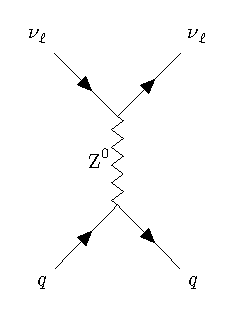
\includegraphics[width=0.3\textwidth]{img/feynman-neutral}\vspace*{2mm}}\hspace{1cm}
  \subcaptionbox{Charged-current neutrino interactions through $\PWpm$ bosons.}{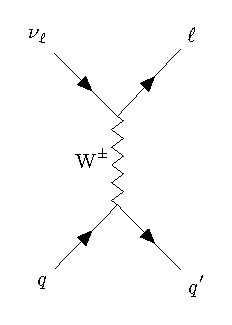
\includegraphics[width=0.3\textwidth]{img/feynman-charged}}
  \caption{Feynman diagrams showing neutrinos $\Pnulepton$ interacting with quarks~$\Pquark$ of nuclei of the ice or nearby rock through $\PZz$ and $\PWpm$ bosons, producing leptons~$\Plepton$ (electrons~$\Pe$, muons~$\Pmu$, tau particles~$\Ptau$) and quarks. Time evolves to the right in these diagrams.}
  \label{fig:Phei1oob}
\end{figure}

These interactions lead to three different kind of event signatures in
the \icecube detector, visualized in figure \ref{fig:eeQuaef6}.

\paragraph{Shower- or Cascade-Like Events}

In both, interactions through \(\PZz\) bosons
(\textit{neutral-current interactions}) and through \(\PWpm\) bosons
(\textit{charged-current interactions}), hadronic showers are created as
energy is transferred from the incoming neutrino to the outgoing quark.
Hadronic showers are particle cascades originating from hadron
particles. If the outgoing lepton is an electron, this may also create
an accompanying electromagnetic shower, which is a particle cascade
originating from particles primarily interacting through the
electromagnetic interaction. \cite{energyreco}

\begin{align*}
  & \text{neutral current:} & \Pnulepton + \text{nucleon} & \rightarrow \Pnulepton + \text{hadron} \ \ \ \ \ \ \Plepton \in \{ \Pe, \Pmu, \Ptau \}                             & \\
  &                         &                             & \rightarrow \Pnulepton \text{ (escapes) } + \text{hadronic shower}  & \\ \\
  & \text{charged current:} & \Pnue + \text{nucleon}      & \rightarrow \Pe + \text{hadron}                                     & \\
  &                         &                             & \rightarrow \text{electromagnetic shower} + \text{hadronic shower}  & \\
\end{align*}

\paragraph{Track-Like Events}

If the outgoing lepton is a muon, this creates track-like event
signatures as muons travel long distances. TeV muons may travel several
kilometers in the antarctic ice. \cite{skysearch, mmc}

\begin{align*}
  & \text{charged current:} & \Pnum + \text{nucleon}      & \rightarrow \Pmu + \text{hadron}                                    & \\
  &                         &                             & \rightarrow \text{muon track} + \text{hadronic shower}              & \\
\end{align*}

\paragraph{Double-Bang Events}

If the outgoing lepton is a tau, the tau will create a track. But the
track will only be a couple of meters long as the tau then decays into
another hadronic shower. This creates a so-called
\textit{double-bang signature}, where two hadronic showers are joined by
a short track. The shorter the joining track is, the more similar the
event looks to a single-cascade-like event.
\cite{skysearch, energyreco, particledatareview}

\begin{align*}
  & \text{charged current:} & \Pnut + \text{nucleon}      & \rightarrow \Ptau + \text{hadron}                                   & \\
  &                         &                             & \rightarrow \text{tau track} + \text{hadronic shower}               & \\
  &                         &                             & \rightarrow \text{hadronic shower} + \text{hadronic shower}         & \\
\end{align*}

\begin{figure}[htbp]
  \centering
  \subcaptionbox{Cascade-like event: The cascade is completely contained within the detector and deposits a total of $1141\TeV$ energy within the detector. Image and data source: \cite{evidence2013,energyreco}}{\halfimage{evidence2013-event-20}}\hfill
  \subcaptionbox{Track-like event: The muon track starts within the detector and deposits a total of $71\TeV$ of energy within the detector before it leaves the detector volume. Image and data source: \cite{evidence2013,energyreco}}{\halfimage{evidence2013-event-5}}\hfill
  \subcaptionbox{Simulated double-bang event: The earlier (red) cascade has been created from the primary neutrino interaction vertex. The tau travels from the position of the first cascade for a short distance, creating a track, before decaying into another later (green) cascade. Image source: \cite{nufact2018}}{\halfimage{nufact2018-double-bang}}\hfill
  \caption{Visualization of examples for the different event signatures of neutrino events observed with \icecube. The spheres represent the energy registered by the respective detector module. The color indexes the time information: Red is the beginning of the event, green the middle, and blue the end of the event.}
  \label{fig:eeQuaef6}
\end{figure}

\subsection{Cherenkov-Light Emission}
\label{sec:cherenkov}

When charged particles, both the primary lepton and particles within the
cascades, move through the detector medium faster than the phase
velocity of light within this medium, they emit so-called
\textit{Cherenkov radiation}, which are photons with wavelengths in the
visible and the near ultra violet spectrum.
\cite{energyreco, instrumentation, skysearch}

The light emission is not isotropic: Photons are emitted under an angle
\(\phi\) relative to the direction of propagation of the charged
particle. \cite{physiklexikon}

\[
  \cos \phi = \frac{1}{\beta\,n} = \frac{c'}{v}, \ \ \ \beta = \frac{v}{c}, \ \ \ c' = \frac{c}{n}
\]

\(n\) is the refractive index of the medium, \(c'\) the speed of light
within the medium, \(c\) the speed of light in vacuum.

The virtual photon field of the charged particle moving through the
medium polarizes the atoms in the medium. Each resulting electric dipole
is a source of electromagnetic radiation. But as each dipole arranges
towards the charged particle, integrating over the whole spatial sphere
around the charged particle, the net emitted radiation vanishes if the
charged particle's velocity \(v\) is smaller than the speed of light
\(c'\) in the medium. For higher velocities, the Coulomb field of the
charged particle can only polarize the atoms within a cone with an
opening angle of \(2\phi\), the \textit{Cherenkov cone}, resulting in a
net photon emission perpendicular to the surface of the cone.
\cite{physiklexikon}

\begin{figure}[htbp]
  \centering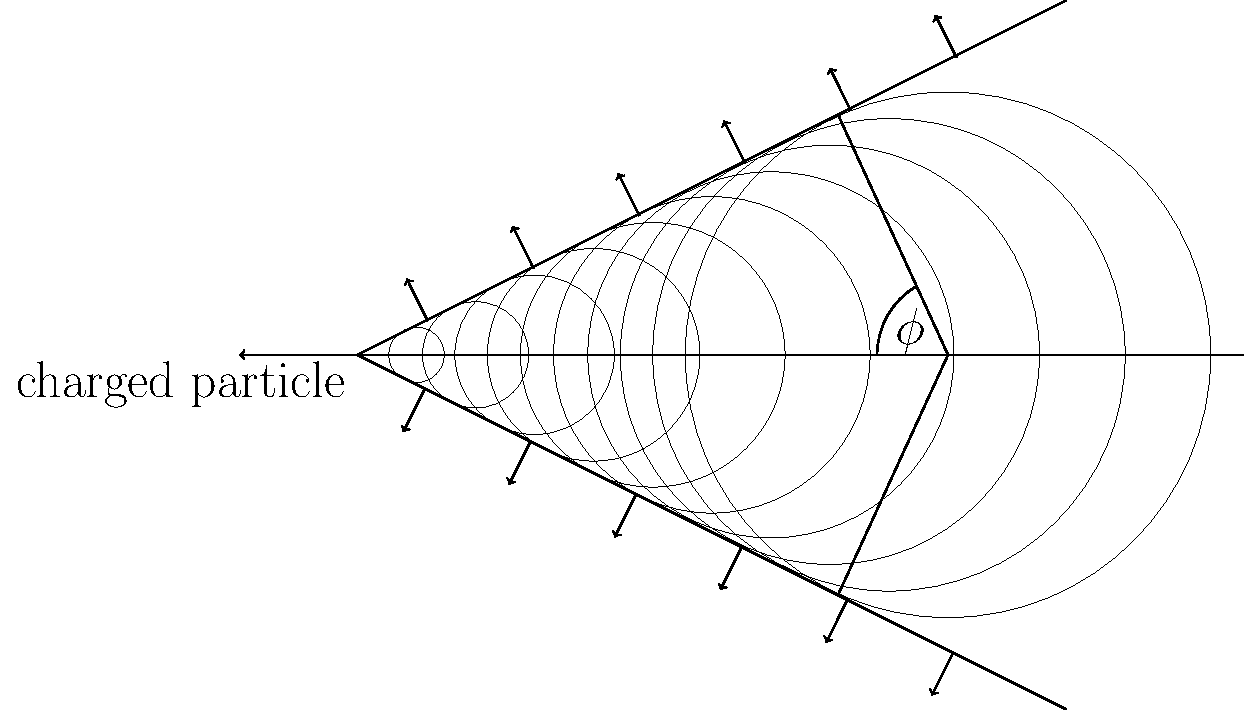
\includegraphics[width=0.5\textwidth]{img/cherenkov}
  \caption{Visualization of the \textit{Cherenkov cone}: A charged particle moves through a medium with a velocity $v>c'$ greater than the phase velocity $c'$ of light within this medium. Due to non-isotropic polarization effects, \textit{Cherenkov photons} are emitted under an angle $\phi$ relative of the direction of motion of the charged particle.}
  \label{fig:ehai2Ahj}
\end{figure}

The spectral distribution of Cherenkov photons is given by equation
\ref{eq:cherenkovspectrum}. A particle with \(\pm z\) elementary charges
that travels a distance \(\d x\) emits \(\d^2 N\) Cherenkov photons with
a wavelength range of \([\nu; \nu + \d\nu]\). \(\alpha\) is the fine
structure constant. \cite{katz2012} The spectrum prefers photons with
shorter wavelengths \(\nu\).

\begin{equation}
  \frac{\d^2 N}{\d x\,\d\nu} = \frac{2\pi\,\alpha\,z^2}{\nu^2}\cdot
  \left( 1 - \frac{1}{\beta^2\,n^2} \right)
  \label{eq:cherenkovspectrum}
\end{equation}

Per GeV of secondary particle shower energy within the detector, an
order of \(10^5\)\nbsp visible Cherenkov photons are created.
\cite{instrumentation}

\subsection{Photon Absorption and Scattering}
\label{sec:scattering}

The propagation of light through a medium depends on the optical
properties of that medium, in particular the velocity of light within
that medium, the scattering probability and the absorption probability.
\cite{lundberg}

The absorption of light for the relevant wavelength range is caused by
electronic and molecular excitation processes \cite{lundberg} and is
quantified by the \textbf{absorption length} \(\lambda\abs\), which is
the mean of the exponentially distributed free path length to absorption
\cite{lundberg}. Therefore, in accordance with the
\noun{Beer-Lambert law}, the absorption length is the path length that
light needs to travel within a medium to have its intensity drop to
\(\sfrac{1}{\e}\) of its original intensity. \cite{lexikonderphysik}
Absorption lengths in the South-Polar ice vary between \(10\m\) in dusty
regions and \(280\m\) in very clear ice layers.
\cite{ackermann, ppcpaper, icepaper}

The scattering of light off microscopic scattering centers, such as
sub-millimeter-sized air bubbles and micron-sized dust grains
\cite{Price1997, ackermann} is the dominant scattering mechanism in
glacial ice \cite{Askebjer1997, lundberg}. This scattering can be
modeled using the more general \noun{Mie scattering} theory, which
describes the scattering of electromagnetic radiation off small,
spherical masses of material with refractive indices differing from the
refractive index of its surroundings.
\cite{Mie1908, ackermann, lundberg}

\noun{Mie scattering} gives the distribution of the scattering angle
\(\theta\) for any wavelength and scattering center size. For ice, this
distribution is approximated using a one-parameter
\noun{Henyey-Greenstein} (HG) phase function
\(p_\text{HG}(\theta; \tau)\), where the one parameter \(\tau\) is the
mean cosine of the scattering angle. \cite{lundberg}

\[ p_\text{HG}(\theta; \tau) = \frac{1 - \tau^2}{2(1 + \tau^2 - 2\tau\, \cos \theta)^\frac{3}{2}}, \ \ \ \tau = \meancostheta \]

The South-Polar ice has shown to be preferentially forward scattering
with a mean cosine of the scattering angle of \(\meancostheta = 0.94\)
with only a weak dependence on the wavelength. \cite{ackermann}

The \textbf{scattering length} \(\lambda\sca\), which is also called
\textbf{geometric} scattering length, is the mean of the exponentially
distributed free path and thereby the average distance between
scatterings. \cite{ackermann} A related and often used quantity is the
\textbf{effective scattering length} \(\lambda\esca\), which is the
distance that light needs to propagate through a turbid medium before
the photon directions are completely randomized. \cite{lundberg}

\begin{equation}
  \lambda\esca = \frac{\lambda\sca}{1 - \meancostheta}
\end{equation}

In a medium with isotropic scattering, the geometric and the effective
scattering lengths are the same. In a preferentially forward scattering
medium like the South-Polar ice, the original direction of a sample of
photons is tendentially retained for several scattering steps until the
photon direction of the sample is isotropized. The projection of the net
velocity vector on the original direction is decreased on average by
\(\meancostheta\) for each scattering. \cite{lundberg}

After \(n\) scatterings, the effectively transported forward distance
along the original direction is
\(\lambda\sca\,\sum_{i=0}^n \meancostheta^i\), such that in the limit of
many scatterings, \(n \rightarrow \infty\), the effectively transported
forward distance becomes the effective scattering length.
\cite{lundberg, ackermann}

\[ \lim_{n \rightarrow \infty} \lambda\sca\,\sum_{i=0}^n \meancostheta^i = \frac{\lambda\sca}{1 - \meancostheta} = \lambda\esca \]

Typical effective scattering lengths within the South-Polar ice are on
the order of \(25\m\) \cite{lundberg} and range from \(5\m\) to \(90\m\)
in the detector volume \cite{icepaper}, corresponding to the geometric
scattering length ranging from \(0.3\m\) to \(5.4\m\).

Light interference effects are ignored during photon propagation as the
average distance between the scattering centers is large compared to the
photon wavelength. \cite{ackermann} Also, despite modeling different ice
regions with abrupt boundaries in the simulations of this study, the
physical boundaries are assumed such that refractive index variations
are continuous. Hence reflection at the medium boundaries is ignored in
simulations. \cite{lundberg}

  \section{Experimental Concepts}
\label{sec:experimental_background}

\subsection{\icecube Detector}

The \icecube neutrino detector is built into a cubic-kilometer of the
glacial ice at Earth's South Pole. 5160 photo detecting optical modules
have been deployed between \(1450\m\) and \(2450\m\) below the surface.
Construction has begun in 2005 with the deployment of the first optical
modules. The detector is fully operational since 2010.
\cite{instrumentation}

The optical modules are anchored on 86 vertical cables called
\textit{strings}, which are positioned on a triangular grid with an
overall hexagonal footprint. The strings are about \(125\m\) apart. Each
string holds 60 optical modules with a vertical spacing of \(17\m\).
\cite{instrumentation}

\begin{figure}[htbp]
  \smallerimage{icecube-schematics-instrumentation}
  \caption{Schematic overview of the \icecube detector. Image source: \cite{instrumentation}}
  \label{fig:aiThai0e}
\end{figure}

Additional to this \textit{in-ice array}, which is designed to measure
neutrinos with energies from the TeV to the PeV scale, the
\textit{DeepCore} sub array hold additional optical modules in order to
lower the detection energy threshold in this region of the detector to
detect neutrinos with energies from \(10\GeV\) to \(100\GeV\).
\cite{instrumentation}

\subsection{Digital Optical Modules (DOMs)}
\label{sec:doms}

The basic detection unit in \icecube is the
\textit{Digital Optical Module} (DOM). Its main components are a photo
multiplier tube (PMT), which detects impacting photons, a main
electronics board, and a flasher board containing light-emitting diodes
(LEDs) for calibration purposes (figure \ref{fig:aK4raigh} a). The DOM's
components are contained within a glass sphere with an outer diameter of
about \(35\cm\) that can withstand high pressures (figure
\ref{fig:aK4raigh} b). The space in between is filled with a gel to
avoid optical effects at the medium boundaries. \cite{instrumentation}

\begin{figure}[htbp]
  \subcaptionbox{Components of the optical module. Image source: \cite{instrumentation}}{\halfimage{dom-components-instrumentation}}\hfill
  \subcaptionbox{Glass sphere containing the components of the optical module. Image source: \cite{gallerynoharness}}{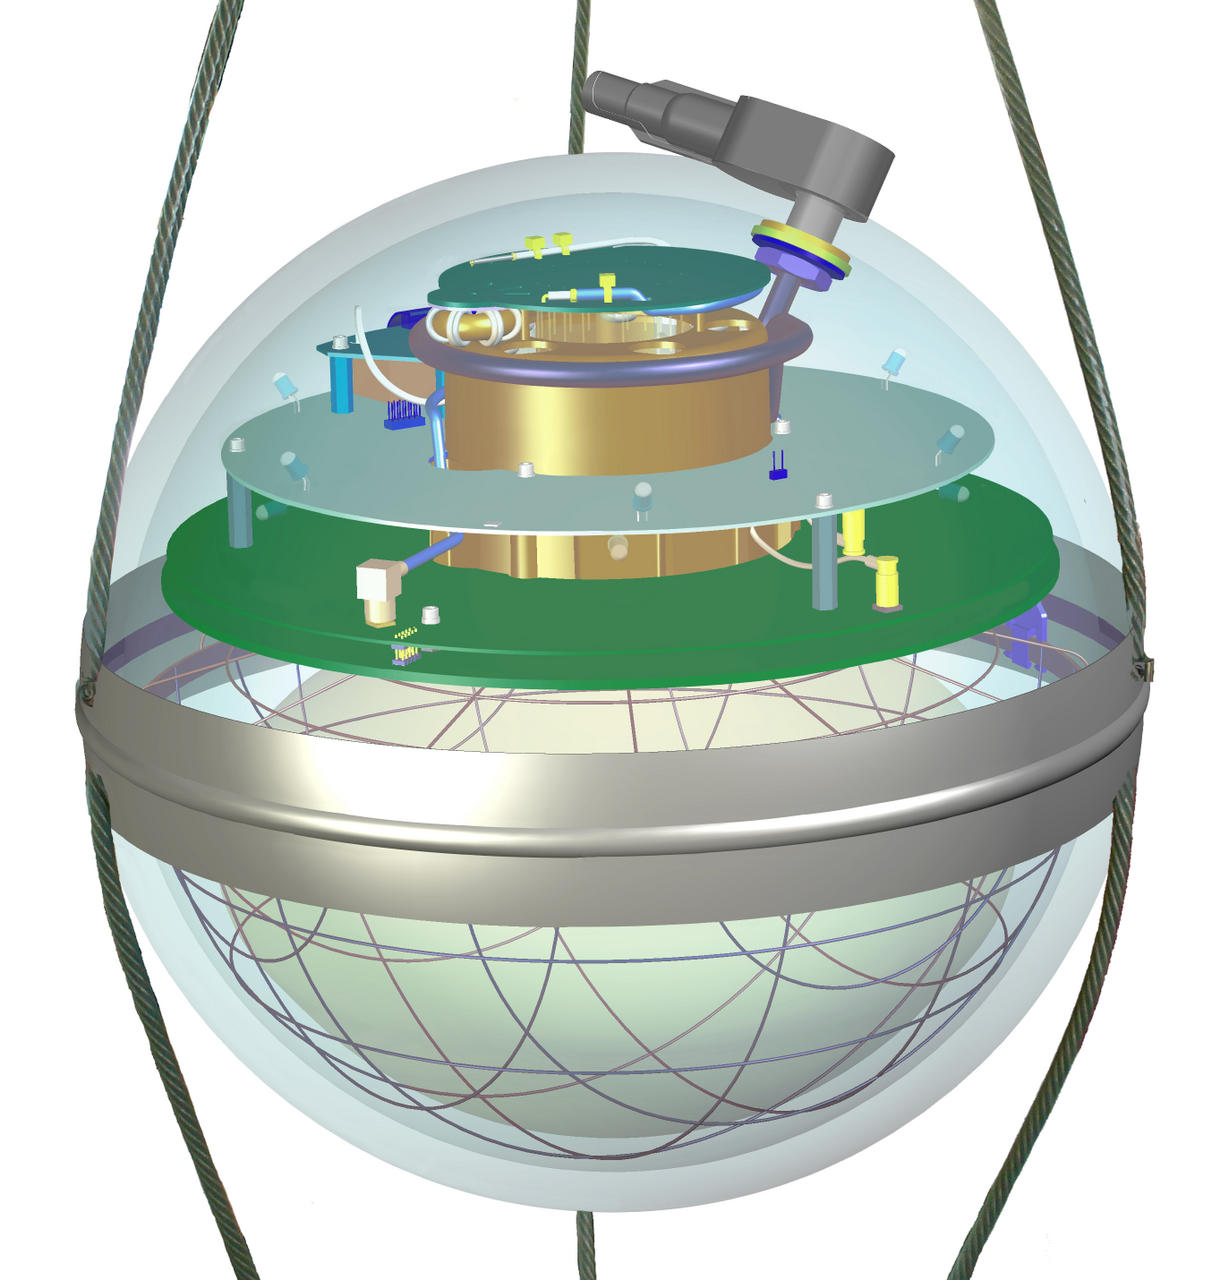
\includegraphics[width=0.35\textwidth]{img/DOMNoHarnessWhiteback_lg-gallery-2013}}
  \caption{Schematic display of a digital optical module (DOM), \icecube's basic detection unit.}
  \label{fig:aK4raigh}
\end{figure}

The recorded signals from the PMT are digitized within the module before
sending the signal to the surface in order to minimize the loss of
information from degradation of analog signals sent over long distances.
\cite{firstyearperformance}

The optical modules are optimized for detecting Cherenkov light emitted
by particles with energies from \(10\GeV\) to \(10\PeV\) up to \(500\m\)
away from the optical module. \cite{instrumentation}

\subsection{Properties of South-Polar Ice}
\label{sec:ice}

The ice at the South Pole has exceptional optical properties, because
air bubbles shrink and vanish under large pressure, forming a so-called
\textit{clathrate hydrate}, where impurities are enclosed inside the ice
crystal structure. \cite{rongenswedishcamera}

Using \icecube's LED flasher calibration system, the properties of
\icecube's glacial ice have been measured: The average distance to
absorption, \(\lambda\abs\), the average distance between successive
scatters \(\lambda\sca\), and the angular distribution of the new
direction after scattering.

To fit these parameters for different depths, the ice has been divided
into \(z\)-layers of an arbitrary thickness of \(10\m\). The ice
parameters have been fitted for each layer such that the properties are
best interpreted as average of their true values over the thickness of
the ice layers. \cite{icepaper}

\paragraph{Scattering}

The measured effective scattering lengths \(\lambda\esca\) range from
\(5\m\) to \(90\m\), corresponding to the geometric scattering length
ranging from \(0.3\m\) to \(5.4\m\). The depth dependence of the
scattering length is shown in figure \ref{fig:Ahxobai3} (a).
\cite{icepaper}

\begin{figure}[htbp]
  \subcaptionbox{Depth dependence of the effective scattering length~$\lambda\esca$ and the effective scattering coefficient~$b_\text{e}:=\sfrac{1}{\lambda\esca}$.}{\halfimage{icepaper-fig-16-esca}\vspace*{2mm}}\hfill
  \subcaptionbox{Depth dependence of the absorption length~$\lambda\abs$ and the absorption coefficient~$a:= \sfrac{1}{\lambda\abs}$.}{\halfimage{icepaper-fig-16-abs}}
  \caption{Values of the absorption length $\lambda\abs$ and the effective scattering length $\lambda\esca$ for different depths, but for a fixed photon wavelength of $400\nm$. Plot taken from \cite[figure 16]{icepaper}. A detailed data table is given in \cite[table C1]{icepaper}.}
  \label{fig:Ahxobai3}
\end{figure}

The wavelength dependence is given by equation \ref{eq:escawavelength}
\cite[section 4]{icepaper}, where
\(b_\text{e} := \sfrac{1}{\lambda\esca}\) is the effective scattering
coefficient, \(\nu\) the photon wavelength, and \(\alpha\) a global fit
parameter. \(b_\text{e}(\nu = 400\nm)\) is given by figure
\ref{fig:Ahxobai3} (a) and \cite[table C4]{icepaper}. The global
parameter \(\alpha\) has been fitted to \(\alpha = 0.90 \pm 0.03\)
\cite[section 5.1]{ackermann}.

\begin{equation}
  b_\text{e}(\nu) = b_\text{e}(\nu = 400\nm) \cdot \left(\frac{\nu}{400\nm}\right)^{-\alpha}
  \label{eq:escawavelength}
\end{equation}

The scattering prefers the forward direction, with a mean cosine of the
scattering angle of \(\meancostheta = 0.94\)
\cite[paragraph 9]{ackermann} (or \(\meancostheta = 0.90\)
\cite{icepaper}).

\paragraph{Absorption}

The absorption lengths in the South-Polar ice vary between \(10\m\) in
dusty regions and \(280\m\) in very clear ice layers. Their depth
dependence is given in figure \ref{fig:Ahxobai3} (b). The absorption
length, which is governed by the dust concentration, is especially low
in the so-called ``dust peak'' at a depth of about \(2000\m\).
\cite{ackermann, ppcpaper, icepaper}

The dependence of the absorption coefficient
\(a := \sfrac{1}{\lambda\abs}\) on the photon wavelength \(\nu\), the
temperature difference \(\delta\tau\) is given by equation
\ref{eq:abswavelength} \cite{icepaper}.

\begin{equation}
  a(\nu) = a_\text{dust}(\nu) + A\,\e^{-\sfrac{B}{\nu}}\, (1 + 0.01 \cdot \delta\tau)
  \label{eq:abswavelength}
\end{equation}\begin{equation}
  a_\text{dust}(\nu) = a_\text{dust}(\nu = 400\nm) \left(\frac{\nu}{400\nm}\right)^{-\kappa}
\end{equation}

The global parameters have been fitted to \(A = (6954 \pm 973)\m^{-1}\),
\(B = (6618 \pm 71)\nm\), and \(\kappa = 1.08 \pm 0.01\)
\cite[section 5.2]{ackermann}.\footnote{The quantity $A$ in \cite{icepaper} corresponds to the quantity $A_\text{IR}$ in \cite{ackermann}. $B$ in \cite{icepaper} corresponds to $\lambda_0$ in \cite{ackermann}.}
The temperature difference \(\delta\tau(d) = T(d) - T(1730\m)\) for
depths \(d\) is given by equation \ref{eq:temperature} \cite{icepaper}.

\begin{equation}
  T(d) = 221.5\unit{K} - 0.00045319\,\frac{\text{K}}{\text{m}}\cdot d + 5.822 \cdot 10^{-6}\,\frac{\text{K}}{\text{m}^2} \cdot d^2
  \label{eq:temperature}
\end{equation}

\paragraph{Ice-Layer Tilt and Ice Anisotropy}

The absorption properties of the ice layers follow the dust
concentration, which does not strictly follow the arbitrary
\(z\)-layers, but is tilted. To model this feature, the ice layers can
also be considered tilted by using an effective-\(z\) coordinate,
\(z_\text{e}(x,y,z) = z + \text{relief}(x,y,z)\), which is shown in
figure \ref{fig:wohr8uaY}. \cite{icepaper}

\begin{figure}[htbp]
  \centering
  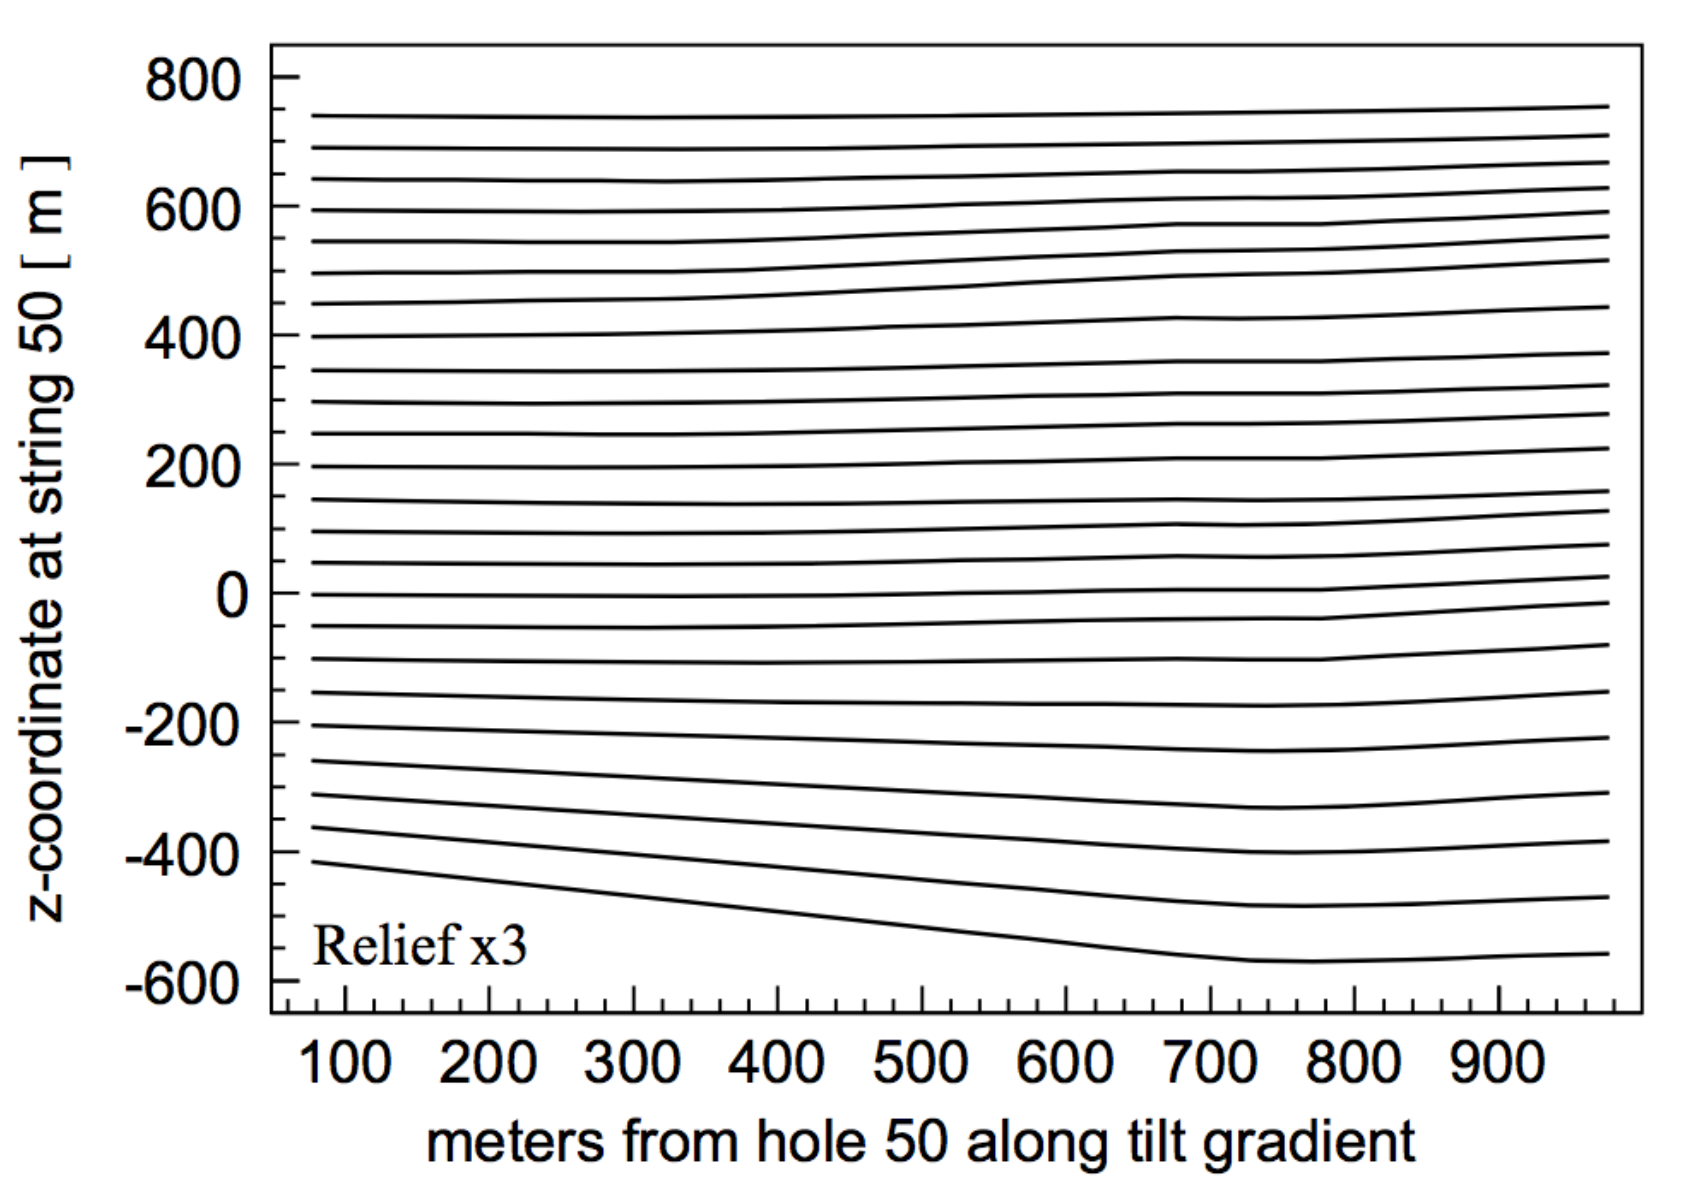
\includegraphics[width=0.5\textwidth]{img/icepaper-fig-14-layers}
  \caption{Ice layers along the average gradient direction within the ice. The relief is amplified by a factor of 3 to enhance the clarity of the layer structure. The lowest layer shown exhibits a shift of $56\m$ between its shallowest and deepest points, which is the largest shift of all layers shown in the figure. Plot and caption taken from \cite[figure 14]{icepaper}.}
  \label{fig:wohr8uaY}
\end{figure}

Furthermore, scattering and absorption show also a slight dependency on
the propagation direction of the photons, aligned with the ice flow
direction of the glacier \cite{icrc17pocam}, which is referred to as
\textit{ice anisotropy}.

This study considers the dependencies of scattering and absorption
length on depth, temperature and wavelength, but does not consider the
ice-layer tilt and the ice anisotropy.

An overview of the different ice models used in \icecube is given in
\cite{flasherdataderivedicemodels}.

\subsection{Hole Ice Around the Detector Strings}
\label{sec:hole_ice}

The so-called \textit{hole ice} is the refrozen water within the drill
holes that were necessary to deploy the detector strings with the
optical modules.

For the \icecube detector, 68 boreholes with an approximate diameter of
\(60\cm\) to a depth of about \(2500\m\) were created using a
\textit{hot-water drilling} technique. Drilling one hole required about
48 hours time. During the deployment, the drill hole was filled with
water. \cite{instrumentation}

When the glacial ice in the drill holes became water, the structures
that were responsible for the specific properties of the bulk-ice layers
were destroyed. Thus, the properties of the hole ice are considered
largely independent of those of the surrounding bulk ice. The deployed
instrumentation become frozen in place and optically coupled to the
surrounding ice sheet when the water in the boreholes became ice again.
\cite{instrumentation}

In order to monitor the freeze-in process, a camera system consisting of
two video cameras in separate spheres, each also equipped with four LEDs
and three lasers, has been deployed along one of the detector strings.
The cameras observed that the drill hole became completely refrozen
within 15 days. \cite{instrumentation}

The camera observations suggest two hole-ice components, a clear outer
region, and an inner column of a smaller scattering length and a
diameter of about \(16\cm\) (figure \ref{fig:daeM6yot}).
\cite{rongenswedishcamera,instrumentation}

\begin{figure}[htbp]
  \centering
  \subcaptionbox{}{\thirdimage{camera2010-01}}\hfill
  \subcaptionbox{}{\thirdimage{camera2010-02}}\hfill
  \subcaptionbox{}{\thirdimage{camera2010-03}}\hfill
  \subcaptionbox{}{\thirdimage{camera2010-04}}\hfill
  \subcaptionbox{}{\thirdimage{camera2010-05}}\hfill
  \subcaptionbox{}{\thirdimage{camera2010-06}}\hfill
  \subcaptionbox{}{\halfimage{swedish-camera-downwards}}\hfill
  \subcaptionbox{}{\halfimage{camera2018-01}}\hfill
  \caption{Monitoring the freeze-in process using a camera system deployed within string number 80. The drill hole freezes from outside in as seen in (a) to (f). The final configuration that can still be observed in 2018 as seen in (h) still shows a diffuse column, called \enquote{bubble column}, on the right-hand side of images (g) and (h). Image sources: \cite{icrc17pocam, camera2010, camera2018}}
  \label{fig:daeM6yot}
\end{figure}

The observed freeze-in process from the outside in is consistent with
the model of \textit{cylindrical freezing}, where impurities or air
bubbles are pushed inwards along the freezing boundaries until they
merge in the center. \cite{rongenswedishcamera} After completing the
freeze-in process, no long-term changes have been observed from 2010 to
2018. \cite{instrumentation, camera2010, camera2018}

In this study, when needing to differentiate between the different
components of the hole ice, the outer clear component will be called
\textit{drill-hole ice}, or \textit{drill-hole column}. The inner
component with a shorter scattering length will be called
\textit{bubble column}. Note, however, that there is no established
nomenclature in the context of \icecube publications, yet.

In this study, the hole-ice columns will be modeled as cylinders. More
complicated geometries such as accounting for the inevitable swinging of
the drilling head, or pressure effects that could lead to a vertical
gradient in the properties of the hole ice, are not considered in this
study.\followup

  \section{Computing Concepts}
\label{sec:simulation_background}

\subsection{Monte-Carlo Simulations of Photons}
\label{sec:monte_carlo}

A Monte-Carlo simulation is a computational method that utilizes a large
amount of random numbers. In order to substitute a complex, possibly
unknown probability distribution, samples of random numbers are drawn
from one or several basic probability distributions and processed in
deterministic calculations. The results are evaluated to gain
information about processes or quantities involved. This method is
especially useful for systems with many degrees of freedom.
\cite{physiklexikon}

This study needs to determine whether and when detector modules are hit
by photons from a given source assuming different ice parameters. In
principle, one could devise a mathematical function of input quantities
and random variables that determines whether and when a photon is
detected by an optical module. This task would be disproportionately
complex, however, especially as the function would have to be revised
for every change in the underlying models.

Therefore, this study uses Monte-Carlo simulations that propagate
photons through the ice in several simulation steps. Based on drawing
random numbers from basic probability distributions, the simulation
determines in each step, whether and when to scatter or to absorb the
photon next, and, in which direction the photon is to be scattered.
Checking for DOM collisions in each step, the simulation is able to
determine for each photon and each detector module whether and when the
photon is detected by the module.

To obtain probability statements from Monte-Carlo simulations, the
\textit{law of large numbers} is employed: If an experiment involving
random processes is repeated \(n\) times, the relative frequency
\(h_n(A):=\sfrac{H(A)}{n}\) of an event\nbsp \(A\), which occurs
\(H(A)\) times in total in these \(n\) experiments, approaches the
\textit{probability}\nbsp \(p(A)\) of the event\nbsp \(A\) for large
numbers\nbsp \(n\) with certainty. \cite{physiklexikon}

\[
  \lim_{n \rightarrow \infty} \text{P}(|h_n(A) - p(A)| < \epsilon) = 1, \ \ \ \epsilon \in \reals
\]

Technical progress concerning computational devices, graphics processing
units (GPUs) in particular, allows to perform highly parallelized
Monte-Carlo simulations on large scale. For a random-walk description of
the propagation of photons, see \cite{absorption1997}. A first
implementation of a photon-propagation simulation through ice is
described in \cite{lundberg}. A study of propagation simulations using
GPUs is presented in \cite{ppcpaper}.

\subsection{Parallel Computing on Graphics Processing Units (GPUs)}
\label{sec:parallel_computing}

Graphics processing units (GPUs) are optimized for performing simple
calculations for a large number of values in parallel.

The general procedure for GPU calculations is to allocate memory on the
GPU, to copy input parameters onto the GPU, perform calculations on the
GPU, and then to download the results from the GPU. This procedure is
efficient if the time that is spent for allocating, and copying to and
from the GPU memory is short compared to the time spent with
calculations on the GPU. \cite{cudacourse}

The basic units for parallelization are \textit{computational threads}.
All operations within a thread are sequential, while all those
operations are applied to a set of threads, called
\textit{thread block}, in parallel. Each GPU may have one or several
thread blocks. \cite{cudacourse}

While technological progress is achieved rapidly, GPU memory is still a
considerably limited resource. In particular fast memory, which requires
a small amount of physical time for reading and writing information, is
expensive. Therefore, memory is divided in several categories: The
\textit{local memory} that belongs only to one thread, is fastest but
most limited. The \textit{shared memory}, which is common to all threads
of one thread block, is slower. Next slower is the
\textit{global memory}, which is common to all thread blocks on the GPU.
Slowest, but in comparison to the GPU memory practically unlimited, is
the \textit{host memory}, which is memory not on the GPU but on other
components of the computer. Efficient memory use is one of the key
concepts for performant GPU programming.
\textit{Coalesce memory access}, which means that each thread in a
thread block reads or writes from or to a coherent memory block parallel
to the other threads of the thread block, increases memory access
performance. \cite{cudacourse}

Techniques that utilize the internal optimizations of GPUs allow for
further performance improvements: Using GPU-native
\textit{atomic operations} such as the increment operator that increases
the value of a variable by 1 is more performant than using a generic
mathematical operation. GPUs support vectors with four components as
native data types. Using \textit{native vectorial operations} such as a
dot product is more performant than implementing the operation as
mathematical function manually. \cite{cudacourse}

In parallel computing, the \textit{step complexity} of an algorithm is a
measure of the physical time the parallelized algorithm needs to run.
The \textit{work complexity} is a measure for the summed computational
work that is done by all threads in that time. A pattern to avoid in
this context is \textit{thread divergence} where some threads have to
stay idle and wait for other threads completing their work.
\cite{cudacourse}


  % Methods:
  % Everything needed to reproduce the work
  \section{Development of Algorithms For the Direct Photon-Propagation Through Hole Ice With \clsim}
\label{sec:methods}

\renewcommand\currentsection{Hole-Ice Algorithms}

\subsection{Modeling Hole Ice as Distinct Cylindrical Ice Volumes}

In the \icecube simulation framework, photon propagation simulation
takes several dependencies into account: The photon absorption length
and the photon scattering length may depend on the photon's wavelength.
Absorption and scattering length may also depend on the photon's
\(z\)-coordinate as the South-Polar ice consists of several
\textit{ice layers}. These ice layers may also be tilted. Furthermore,
the absorption length may depend on the photon's direction of motion,
which is called \textit{absorption anisotropy}.

This study adds another ice feature to the simulation: Hole ice may be
modeled by adding cylinder-shaped volumes within the surrounding bulk
ice where the propagation properties, or, to be specific, the photon's
absorption length and scattering length, differ from the propagation
properties of the bulk ice.

Figure \ref{fig:aiw2Thah} illustrates such a scenario for one single
photon: The photon's trajectory starts in the bulk ice. The photon
enters the hole-ice cylinder where the scattering length is shorter as
in the bulk ice. Hence the photon scatters more frequently within the
cylinder. When the photon leaves the hole-ice cylinder the propagation
properties of the bulk ice take effect again, resulting in the photon
scattering less frequently after leaving the cylinder.

\begin{figure}[htb]
  \centering
  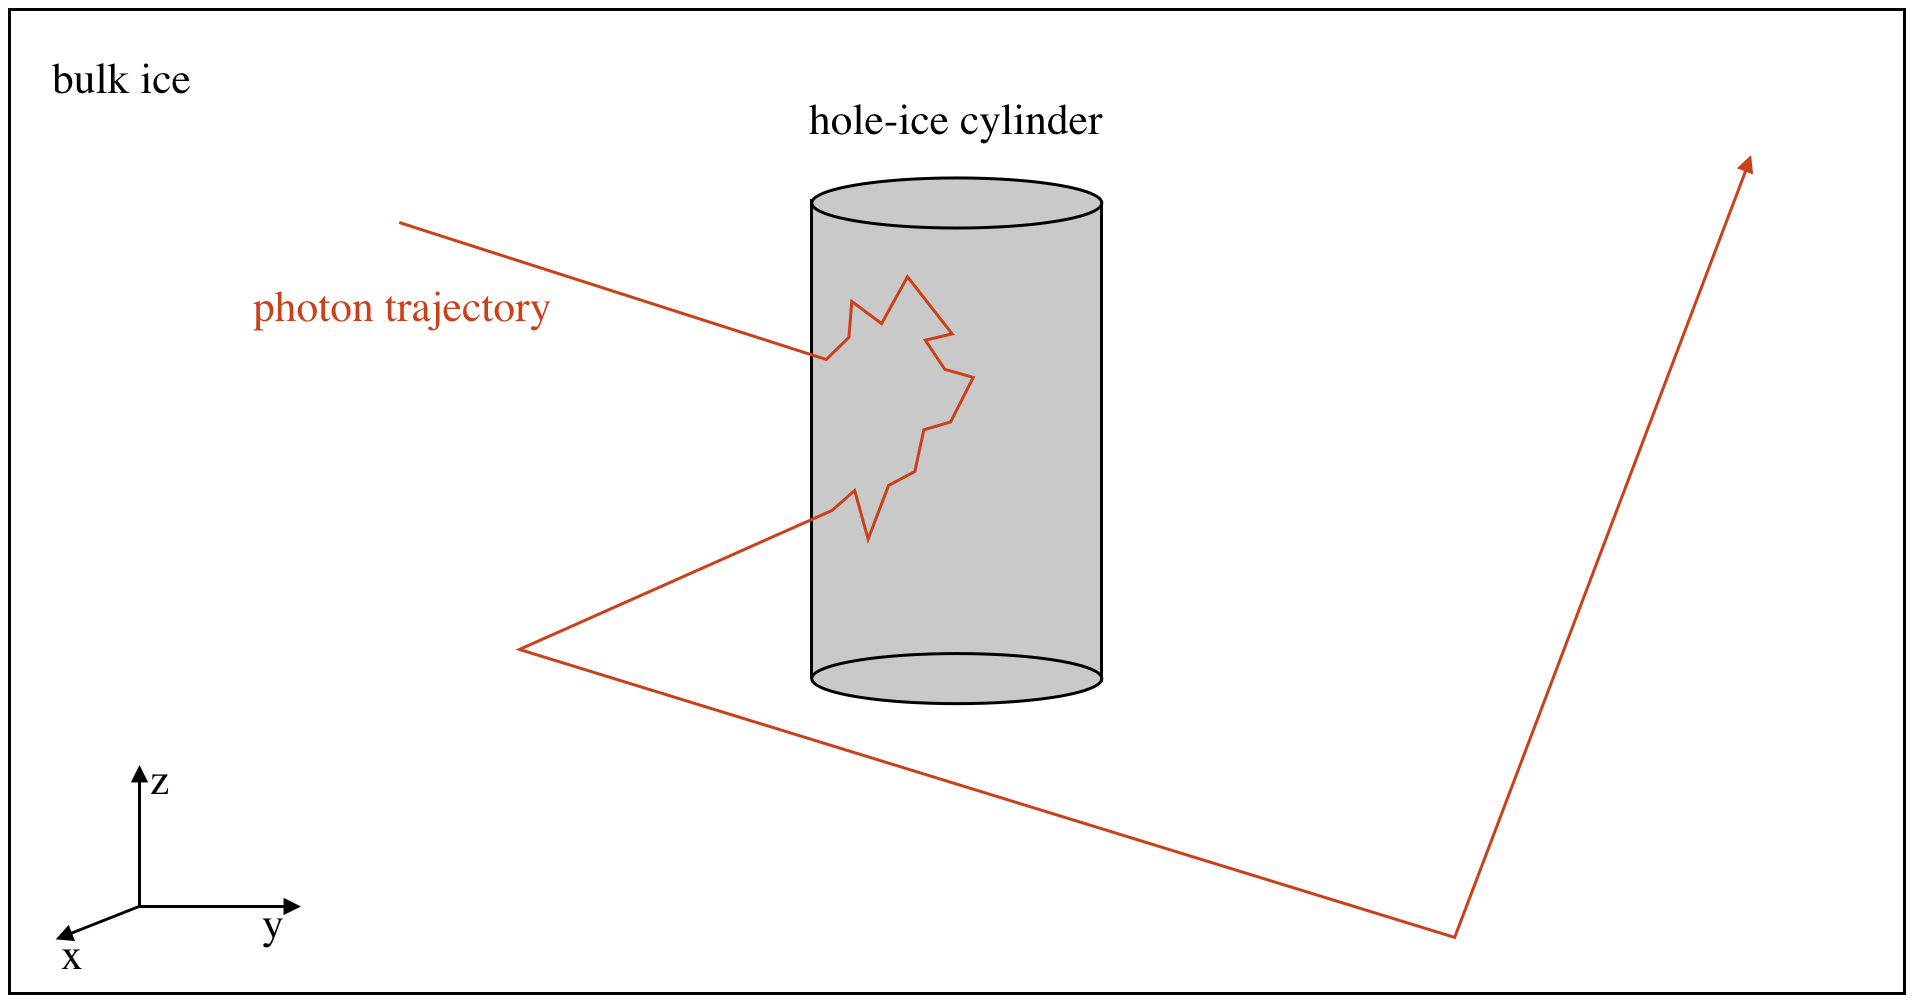
\includegraphics[width=0.6\textwidth]{img/hole-ice-as-cylinder-shaped-areas}
  \caption{Schematic diagram of a propagating photon. The photon enters a hole-ice cylinder with a scattering length different from the outside ice. When leaving the cylinder the photon assumes the scattering length of the outside ice again.}
  \label{fig:aiw2Thah}
\end{figure}

In this study, cylinders are always defined along the \(z\)-axis. Also,
the scattering angle is assumed to behave the same within the hole ice
as in the bulk ice.

  \subsection{Propagating Photons Through Different Media}

\subsubsection{Very Basic Photon-Propagation Algorithm}

A first, very basic photon-propagation algorithm, which is not actually
implemented in \clsim, but is presented as comparative example, moves
the photon by a small distance \(\delta x\). At the new photon position,
the algorithm checks for detection at an optical module and randomizes
as a function of the scattering and absorption lengths whether the
photon should be scattered or absorbed by the ice at this position.
Then, the photon is propagated again by the same small distance
\(\delta x\). The same loop repeats until the photon either hits an
optical module or is absorbed by the ice. Figure \ref{fig:ieph6Bie}
illustrates a propagation scenario in a two-dimensional coordinate
system. Figure \ref{fig:ohsa0miG} presents the algorithm as flow chart.

\begin{figure}[htb]
  \smallerimage{photon-trajectory-naive-ieph6Bie}
  \caption{Illustration of a basic photon-propagation algorithm in a two-dimensional coordinate system. The photon is propagated by a small distance in each propagation step. At each position, the algorithm checks for absorption, scattering and whether an optical module has been hit.}
  \label{fig:ieph6Bie}
\end{figure}

\begin{figure}[p]
  \image{algorithm-naive-propagation}
  \caption{Flow chart of a basic photon-propagation algorithm. Interfaces, where the algorithm begins or ends, are displayed as violet pill shapes. Processes, where the algorithm performs an operation or a calculation, are displayed as brown rounded boxes. Decisions are displayed as green rounded diamond shapes. One propagation step consists of moving the photon by a fixed small distance $\delta x$, checking for detection as well as randomizing scattering and absorption within the ice.}
  \label{fig:ohsa0miG}
\end{figure}

This very basic propagation algorithm can handle propagation through
different media just by making the scattering and absorption
probabilities depend on the current photon position and direction. Ice
layers and ice layer tilt can be implemented by making the scattering
and absorption probabilities depend on the current photon position,
absorption anisotropy by making the absorption probability depend on the
current photon direction as well. Hole-ice cylinders can be implemented
by checking whether the current photon position is within any of a list
of cylinders defined in any way, either by supplying a list of cylinder
coordinates and radii, or by re-using the coordinates of the detector
strings.

This basic propagation algorithm, however, is very inefficient regarding
computational performance: The algorithm moves the photon over long
distances in small steps without changing the direction. For a typical
geometric scattering length of two meters, moving the photon in steps of
\(\delta x = 1\mm\) per propagation step would mean performing 2000
propagation steps before changing the direction of motion.

The propagation algorithm can be made more efficient by moving the
photon in each propagation step not by a small distance \(\delta x\) but
by the whole distance to the next interaction point. This way, the above
example would take only one propagation step rather than 2000. This
performance improvement, however, comes at the cost that propagating
through different media requires a different, more involved
computational approach. This more efficient propagation algorithm, which
is the standard photon-propagation algorithm in \icecube, will be
described in the next section.

\subsubsection{Standard Photon Propagation Algorithm}
\label{sec:standardphotonpropagationalgorithm}

\label{sec:standard_photon_propagation_algorithm}
\label{sec:standard_clsim}

In \icecube's standard photon-propagation algorithm, a propagation step
moves the photon not just by a small, fixed distance \(\delta x\) but to
the next interaction point at once. An interaction may be the photon
scattering within the ice, the photon being absorbed by the ice, or the
photon hitting an optical module. \cite{clsimsource, ppcpaper}

At each scattering point, the algorithm randomizes the new photon
direction based on the scattering angle distribution, and how far the
photon will travel until it is scattered again based on the scattering
length. How far the photon will travel until it is absorbed is
randomized just once when the photon is created.

For each propagation step, the algorithm checks whether the photon will
hit an optical module on the path between two scattering points. Also,
the algorithm checks whether the destined distance to absorption will be
reached before the next scattering point. If the photon will be
destroyed in this step, either by being absorbed in the ice, or by
hitting an optical module, the final position is recorded. Otherwise,
the photon proceeds to the next scattering position. This loop is
repeated until the photon is either absorbed or hits an optical module.
\cite{ppcpaper}

Figure \ref{fig:Ar0vai8u} shows a flow chart of this algorithm. Figure
\ref{fig:oheeL3ai} shows the same two-dimensional scenario as figure
\ref{fig:ieph6Bie} in the previous section, but illustrates how the same
photon trajectory is modeled by this algorithm with significantly less
simulation steps.

\begin{figure}[htbp]
  \smallerimage{photon-trajectory-oheeL3ai}
  \caption{Illustration of \icecube's standard photon-propagation algorithm in a two-dimensional coordinate system. The photon is propagated from one scattering point to the next scattering point in each propagation step. In each step, the algorithm checks for absorption and whether an optical module (DOM) is hit in between the two scattering points.}
  \label{fig:oheeL3ai}
\end{figure}

\begin{figure}[p]
  \image{algorithm-photon-propagation}
  \caption{Flow chart of the standard photon-propagation algorithm. One propagation step consists of moving the photon from one scattering point to the next scattering point. If the photon hits an optical module in between the two scattering points, the algorithm records a hit and destroys the photon. If the photon is absorbed in the ice in between the two scattering points, it will only be propagated to the position of absorption and it will not reach the next scattering point. When adding propagation through hole ice with a different scattering length to this algorithm, the calculation of the next scattering point needs to be modified accordingly.}
  \label{fig:Ar0vai8u}
\end{figure}

Assuming the number of calculations in each scattering step is of the
same order of magnitude in both described algorithms, the number of
simulation steps translates to the total number of calculations the
processing unit needs to perform for each photon. Thus, the algorithm
that needs much less simulation steps is also much more efficient.

Propagating a photon through several media with different optical
properties is more involved in this algorithm than in the basic one. If
the algorithm calculates the distance to the next interaction point
considering only the interaction properties of the ice at the current
position of the photon as suggested by the basic algorithm, then the
next interaction point would be calculated inaccurately if the medium
properties change between two interaction points. The larger the
scattering length gets compared to the size of the ice volumes with
constant interaction properties, the worse the inaccuracies become. This
can be illustrated by an extreme example where the scattering length and
the absorption length within the bulk ice are several meters long, but
the photon would hit a cable with a diameter of only a couple of
centimeters between two scattering points. The cable would absorb the
photon at once. But if the next interaction point is calculated
evaluating only the interaction properties at the position of the
current scattering point, then the photon ignores the cable and
continues on its path without being absorbed by the cable.

The solution to this problem chosen for the standard propagation
algorithm in \icecube is to implement medium transitions in the
following manner: Rather than randomizing the geometrical distance
\(X:=\overline{AB}\) from the current interaction point \(A\) to the
next interaction point \(B\) itself, the algorithm randomizes the number
\(N :\in \reals^+\) of interaction lengths the photon will travel to the
interaction point, like a budget. This budget is spent by considering
the different media on the way from the current interaction point along
the photon's direction, and converting the number of interaction lengths
into a geometrical distance according to the shares of the different
media in the path of the photon between the two interaction points.

Suppose, starting at interaction point \(A\), the photon travels in
\(m :\in \naturals\) media \(M_i\) with interaction lengths
\(\lambda_i\) for a distance of \(x_i\) respectively until it reaches
the next interaction point \(B\). In each medium \(M_i\), the algorithm
spends \(n_i: x_i = n_i\,\lambda_i\) of the budget \(N:=\sum_1^m n_i\)
that has been randomized at interaction point \(A\) until it reaches
interaction point \(B\) in a distance \(X:=\overline{AB}\).

\begin{equation}
  X = \sum_{i=1}^m x_i = \sum_{i=1}^m n_i\,\lambda_i, \ \ \ \ N = \sum_{i=1}^m n_i
  \label{eq:convertbudgettodistance}
\end{equation}

Each distance \(x_i\) is the length of the trajectory the photon spends
in medium \(M_i\). The first distance \(x_1\) is the distance from the
starting point \(A\) to the medium border of \(M_1\) and \(M_2\) along
the photon direction. The subsequent distances \(x_i\) are the distances
of the first medium border (of \(M_{i-1}\) and \(M_i\)) and the second
medium border (of \(M_i\) and \(M_{i+1}\)) respectively along the photon
direction. The last distance \(x_m\) is determined by how much of the
budget \(N\) is left in the last medium, \(x_m = n_m\,\lambda_m\), such
that the overall budget \(N:=\sum_{i=1}^m n_i\) is spent.

Coming back to the extreme example where a cable lies ahead on the
photon path, the algorithm now considers all media on the path along the
photon direction in order to convert the number of interaction lengths
into a geometrical distance to the interaction point. As the absorption
length within the cable's medium is set to zero, all of the
absorption-length budget is spent at the medium border to the cable,
resulting in the final interaction point of the photon being right at
the point where the photon enters the cable. Thus, this algorithm lets
the photon be absorbed by the cable as intended.

Ice layers, the tilt of the ice layers, and the absorption anisotropy
are modeled in this algorithm by implementing the rules on how the
interaction budget is spent accordingly. Adding cylinder-shaped volumes
to model hole ice or cables means to further extend these rules on how
the scattering and absorption budgets are spent along the photon's
trajectory.

Two different algorithms for the photon propagation through
cylinder-shaped volumes are described in the following sections: Section
\ref{sec:algorithm_a} describes a first approach where the propagation
through the hole-ice cylinders is added as subsequent correction for the
existing medium-propagation algorithm. Section \ref{sec:algorithm_b}
describes a second approach where the existing medium-propagation
algorithm is rewritten in order to support the propagation through
hole-ice cylinders the same way as other medium transitions.



  \include{text/gliederung}


  %\include{text/cross_checks}
  %\include{text/likelihood}
  %%!TEX root = ../diplomarbeit.tex

\section{Calculating intersections of photon trajectories with hole-ice cylinders}

In order to make the hole-ice simulation more efficient, one needs to calculate the intersection points of the photon trajectories with the hole-ice cylinders.

\image{intersection-Kahm4UeY.pdf}

\lipsum

  %\subsection{Hole Ice Trajectory
Corrections}\label{hole-ice-trajectory-corrections}

Consider a random photon trajectory through the ice. The photon is
created by a particle interaction at the starting point of the
trajectory. On its way, the photon is scattered several times within the
ice before it is absorbed and thereby detected in one of IceCube's DOMs.

\image{photon-trajectory-oheeL3ai.pdf}

\begin{itemize}
\item
  Consider path of photon through ice.
\item
  Interaction propability determined by ice properties and photon
  wavelength.
\item
  Interaction points determined by these properties and random process.
\item
  Look at part of this trajectory, A B between two interactions.
\item
  Change scenario by adding hole ice cylinder.
\item
  Determine how the trajectory is affected by this.
\item
  Consider a photon trajectory through the ice that partially goes
  through hole ice.
\item
  Within hole ice, the ice properties are different from outside.
\item
  Most notably, the impurities (dirt) cause the photons to scatter or be
  absorbed more often there.
\item
  I.e. Scattering and absorption coefficients are larger within hole
  ice.
\item
  Correspondingly, the scattering and absorption lengths, which are the
  mean free distances until scattering or absorption, are shorter.
\end{itemize}

\image{photon-trajectory-aiph6ahD.pdf}

\begin{itemize}
\tightlist
\item
  Consider simulation of a photon.
\item
  \(A\) is the last point of interaction, i.e.~fixed.
\item
  \(B\) is determined by random process.
\item
  Consider a scenario where a photon trajectory starts at point \(A\)
  and ends at point \(B\), where it is scattered or absorbed. The photon
  does not interact inbetween \(A\) and \(B\).
\end{itemize}

\image{photon-trajectory-Edahi9sh.pdf}

\begin{itemize}
\tightlist
\item
  Now, change scenario: add hole ice cylinder.
\item
  Due to locally increased interaction coefficients, the free path is
  shorter, i.e.~modified \(B\).
\item
  Why is the path shorter?
\item
  B is determined by random variable.
\item
  If the mean free path is shorter (because the likelyhood if
  interaction is larger), then the random variable is smaller.
\item
  The change is \(\Delta b:= \overline{AB'} - \overline{AB}\).
\end{itemize}

  %\section{Problems}\label{problems}

\begin{itemize}
\tightlist
\item
  numerical issues where dependent information are calculated using
  different formulae. Methematically, both ways must lead to the same
  result; but numerically, both can differ, which leads to conflicts in
  the simulation. See 2018-01-16.
\item
  \textbf{Sonderfall: Teilchen fliegt in z-Richtung}: Diesen Fall habe
  ich die ganze Zeit über nicht berücksichtigt und lasse das auch
  einstweilen bleiben. (2018-01-16)
\end{itemize}

  %
  %%Foo \cite{mueller2000}
  %%\printbibliography
  %
  %\appendix
  %%!TEX root = ../../diplomarbeit.tex
\section{Calculating intersection points with SymPy}
\label{app:calculating_intersections_with_sympy}

\todo{Github reference}

To verify this result, this calculation can be repeated using computer algebra systems. The following listing shows how this could be done with \textbf{SymPy}\footnote{\textbf{SymPy} is a Python library for symbolic mathematics. \url{http://sympy.org}} .......

\pythoninput{../Logbuch/2018-02-13_schnittpunktberechnung.py}


\end{document}